\documentclass{article}
\usepackage[super]{natbib}
\usepackage{enumitem}
\usepackage{float}


% Language setting
% Replace `english' with e.g. `spanish' to change the document language
\usepackage[english]{babel}

% Set page size and margins
% Replace `letterpaper' with `a4paper' for UK/EU standard size
\usepackage[letterpaper,top=2cm,bottom=2cm,left=3cm,right=3cm,marginparwidth=1.75cm]{geometry}

% Useful packages
\usepackage{amsmath}
\usepackage{graphicx}
\usepackage{authblk}
\usepackage[colorlinks=true, allcolors=blue]{hyperref}

\renewcommand\Authfont{\fontsize{9}{10.4}\selectfont}

\title{%
  Masa Protocol \\
\bigskip
  \large Soulbound identity infrastructure for building web3 communities
  }
\author{Brendan Playford, Calanthia Lan Mei, Sebastian Gerske, Miquel Cabot}
\date{May 11, 2023} % Set the desired date to published date

\begin{document}

\maketitle

\vspace{0.2cm}

\begin{abstract}
    The Masa Protocol addresses the need for a scalable, interoperable, and standardized on-chain identity infrastructure for the rapidly evolving web3 ecosystem. Recognizing the multi-dimensional nature of identity, Masa proposes an open framework with programmable privacy at its core. Utilizing Soulbound Tokens (SBT) as identity primitives, the protocol enables a dynamic representation of an individual's identifiers, encompassing credentials, affiliations, behaviors, reputation, and social roles. Masa's decentralized oracle network facilitates cross-chain data interoperability, private data management, governance, and account abstraction. Deployed on five leading EVM-compatible blockchains, the Masa Protocol has generated over 1,200,000 identifiers for more than 500,000 individuals (at the time of publishing), demonstrating the potential of SBTs in establishing identity, provenance, and reputation in web3.
\end{abstract}

\section{Introduction}

As the world transitions from traditional web2 architectures to the decentralized web3 landscape, there is an increasing demand for scalable, interoperable, and standardized on-chain identity infrastructure. Identity infrastructure is essential for establishing and maintaining digital identities, facilitating secure interactions, and enabling rich, multi-dimensional data representation for billions of users. Existing solutions, such as Verifiable Credentials (VCs) and Decentralized Identifiers (DIDs), have limitations in usability, interoperability, and programmable privacy, leading to a fragmented on-chain identity ecosystem. To address these challenges and to harness the potential of web3, we present the Masa Protocol.
\\
\newline
The Masa Protocol is designed to provide an open, easy-to-implement framework for identity in web3, with an open data standard and programmable privacy at its core. Masa lays the foundation for Vitalik’s vision for Soulbound Tokens (SBT) as identity primitive for a Decentralized Society (DeSoc)\cite{vitalik2022}. Through a range of identity primitives, Masa enables the representation of an individual's complex, ever-changing, set of identifiers, which includes \emph{credentials, affiliations, behaviors, reputation, and social roles}. This holistic approach to digital identity empowers users to control their data and ensures continuity as identifiers evolve over time.
\\
\newline
Masa's decentralized oracle network offers cross-chain data interoperability, private data management, governance, and account abstraction, thereby streamlining the integration of web3 identity into diverse applications. Deployed on five leading EVM-compatible blockchains, the Masa Protocol has generated over 1,200,000 identifiers for more than 500,000 individuals (at the time of publishing) at the time of publishing, showcasing its potential to revolutionize web3 identity as the de-facto identity infrastructure for developers building web3 communities.
\\
\newline
In this whitepaper, we will outline the architecture, design principles, and functionalities of the Masa Protocol, and discuss its implications for the future of digital identity in web3. Our aim is to demonstrate how the Masa Protocol can unlock new possibilities for decentralized applications, drive user adoption, and advance the vision of a truly decentralized society.
\section{Identity primitives }

\subsection{Soulnames}
A soulname is a domain name or handle for a soul in web3. They are human-readable pseudonymous usernames or handles that resolve to a user’s wallet containing the soulname. Soulnames are letters, numbers, and/or emojis soulnames represent a person's persona and affiliation with a community – affiliations are linked by appending a top-level domain suffix in the following form: username.suffix. 
\\
\newline
For example, Masa’s .soul domain name holders are affiliated with the Masa community and are members of Masa Societies. Celo’s .celo domain represents an affiliation to the Celo community and the community's values, along with an individual's expression of their persona through the username. 
\\
\newline
At Masa, we have conviction that web3 users, and people in general, have deeply rooted psychological behavior that binds them to a community, and as such, people seek to present this affiliation in web3 through a pseudonymous persona – soulname – that reflects a person's core values, and beliefs. 
\\
\newline
Soulnames are tradable and based on ERC-721; they compose with the Masa SoulLinker to resolve addresses and link to SBT identifiers such as Masa Green, proving a user is not a bot to 99.6% efficacy. They are simple to mint and transfer like an NFT and once transferred, they resolve to the new wallet holding the NFT instantly. 
\\
\newline
Being simple to mint and register, soulname minting can be embedded natively within an app such as a web3 game or NFT platform, providing a viable source of revenue. Soulnames can be traded on platforms like OpenSea to provide secondary market value to holders. ENS-based domain services require more steps for a user to register and transfer ownership, making them unsuitable for many fully integrated use cases. Soulnames can be used in apps and wallets as identifiers, usernames, and handles and resolved to addresses in wallets for making payments to another individual without sharing a 42-character hexadecimal address with the sender.  
\subsection{Soulbound Tokens (SBTs)}
\subsubsection{Introduction}
Non-Fungible Tokens (NFTs) have gained widespread usage as an incentive for web3 community building. However, they exhibit limitations in long-term, sustainable community building due to short-term hype cycles and diminishing loyalty. Soulbound Tokens (SBTs), in contrast, promote long-term community building as they are non-transferable and reward users for desired actions and complex ecosystem interactions. 
\\
\newline
NFTs often lack utility and are not designed to be interconnected or tied to a user's identity; being transferable accelerates user churn and the inevitable dumping of NFTs in illiquid markets. SBTs, however, serve as functional utility tokens, inherently connected to a user's web3 identity, and can be stacked to create an incrementally more detailed identity and reputation that is not possible with NFTs. 
\\
\newline
Masa’s SBTs offer gas savings compared to NFTs, and as such, can be issued cost-effectively to users. Moreover, SBTs are economically scalable by design, enabling projects to grow their community without diluting the value of transferable assets used to reward and honor members; thereby representing tokenized loyalty on-chain.
\\
\newline
NFTs still present regulatory challenges, as they are taxed in various jurisdictions, creating tax issues for users and the issuers, whereas SBTs do not share these regulatory concerns and can be utilized to build and grow web3 communities in a low-risk manner.
\\
\newline
Soulbound Tokens (SBTs), as suggested by Ethereum creator Vitalik Buterin, are an innovative concept that can help establish the foundation for a Decentralized Society (DeSoc). SBTs are non-transferable NFTs, meaning they cannot be bought, sold, or traded, and are permanently associated with a particular user's blockchain account, usually an Ethereum or EVM-based wallet.
\\
\newline
\subsubsection{Example use cases}
\begin{enumerate}[label=\arabic*.]
    \item Rewards and loyalty: Masa soulbound badges represent a user’s status and contribution in a web3 community. Community builders and developers can leverage these soulbound badges to identify power users, offer SBT-gated perks, and gamify community engagement.
    \item Compliance and anti-bot: The Masa Wallet Screening SBT ensures that users meet compliance and regulatory requirements, such as anti-money laundering (AML) and counter-terrorist financing (CTF) rules. The Masa Green SBT proves that a wallet is not a bot and serves as a soulbound verification method.
    \item Credit and underwriting: The Masa Credit Score SBT allows users to build credit scores based on their financial behavior and activities on the blockchain, enabling better access to credit and other financial services.
    \item Reputation and DAO participation: Using SBTs, users can establish and maintain a reputation within their ecosystem of choice using various SBTs to represent their credentials, contributions, and affiliations, and participate in Decentralized Autonomous Organizations (DAOs) or a native on-chain community.
  \end{enumerate}

Masa has extended the ERC-721 standard to cater to the unique requirements of SBTs, providing a comprehensive interface for the development and implementation of these tokens. This new standard, EIP-SBT, aims to standardize the SBT concept across the Ethereum ecosystem, making it easier for developers to create and deploy SBTs for various applications
\subsubsection{EIP-SBT}
EIP-SBT introduces a standard interface for Soulbound Tokens (SBTs), which are non-transferable identifiers that, when composed together, form a complete identity for an individual. Identifiers represent physical and interpersonal characteristics not wholly shared with any other person, such as credentials, affiliations, behaviors, reputation, and social roles. 
\\
\newline
The following standard allows for the implementation of a standard API for SBTs within smart contracts. This standard provides basic functionality to mint, track and burn SBTs, resulting in a gas saving of 38\% on the deployment and 3\% on the minting over EIP-721.
\\
\newline
This EIP outlines an interface inspired by the EIP-721 standard for creating Soulbound tokens. However, it does not inherit from the EIP-721 standard to establish a new token type as shown in Appendix \ref{app.eipsbt}.
\begin{figure}[h]
    \centering
    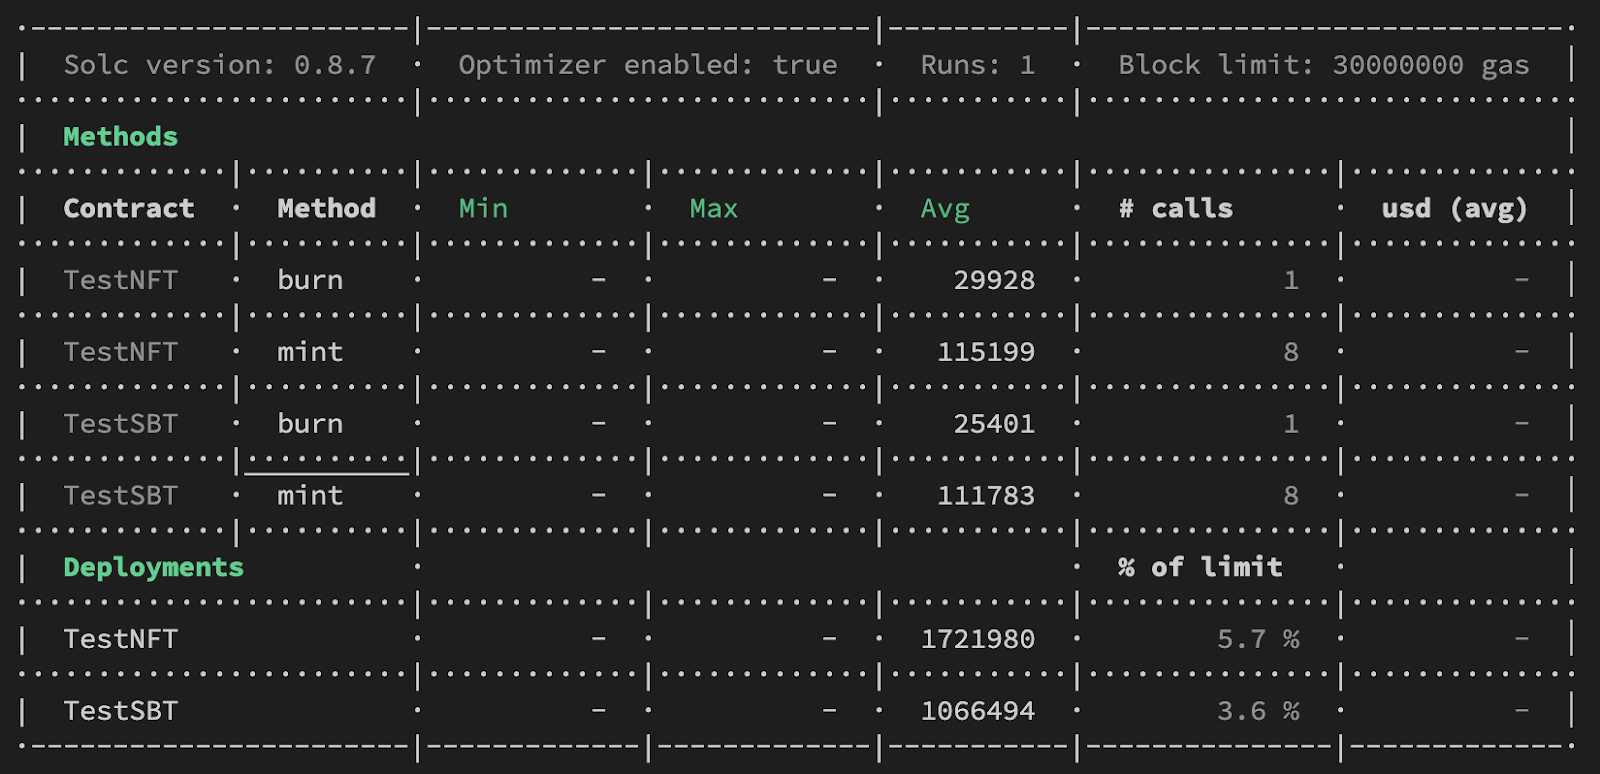
\includegraphics[width=0.8\textwidth]{gas-usage.png}
    \caption{Masa SBT gas usage comparison to ERC-721}
  \end{figure}
\subsubsection{Authority Soulbound Tokens (ASBTs)}

An Authority Soulbound Token (ASBT) inherits from EIP-SBT and adds a specific minting role wherein the minting process is confined exclusively to authorized parties, often referred to as issuers or authorities. These entities hold the role that enables the creation of new SBTs. In a typical ASBT framework, an end-user submits a request or completes an action wherein the designated authority or issuer mints a new token on behalf of the user to their wallet – paying for both the gas and the Masa Protocol fee in Masa Tokens. To ensure that only authorized issuers have the ability to mint new tokens, a modifier is incorporated into the \texttt{mint()} function of the ASBT. This modifier is designed to verify that the caller of the function possesses the minter role, thereby maintaining the integrity of the minting process.

\begin{verbatim}
onlyRole(MINTER_ROLE)
\end{verbatim}

\subsection{Self Sovereign SBTs (SSSBTs)}

The second type of Soulbound Token (SBT) is the Self Sovereign SBT (SSSBT). In these SBTs, authorities or issuers issuing an attestation are required to sign an EIP-712 message using the ECDSA algorithm, allowing the end-users to mint new, verified, tokens independently. When the end-user invokes the mint function, the smart contract verifies that the user has passed a valid signature authorized by the issuer, which ensures that the user has not tampered with the attestation signed by the authority. During the minting process, the smart contract checks the signer's validity and the accuracy of the signature. To achieve this, a \texttt{verify()} function is implemented.

\begin{verbatim}
solidity
Copy code
function _verify(
    bytes32 digest,
    bytes memory signature,
    address signer
) internal view {
    address _signer = ECDSA.recover(digest, signature);
    if (_signer != signer) revert InvalidSignature();
    if (!authorities[_signer]) revert NotAuthorized(_signer);
}
\end{verbatim}
This approach ensures that the minting process remains secure and that only authorized issuers can enable end-users to create new tokens, thus preserving the integrity of the Self Sovereign Soulbound Token (SSSBT) mechanism.

\subsection{Zero-Knowledge Soulound Tokens (zkSBT)}

The Masa zkSBT (Zero-Knowledge Soulbound Token)\cite{zksbt} is a brand-new token design that provides privacy-preserving and secure storage of private data on any EVM blockchain. The zkSBT inherits from the Masa SBT Self-Sovereign token standard, and is designed to store private user data in an encrypted and secure manner. Masa’s zkSBT will be released in Q2 2023 for community development, and a detailed academic paper will be published detailing the zkSBT implementation.
\\
\newline
The zkSBT contract is designed to provide privacy and security for users' private data while maintaining the benefits of decentralized data storage. By utilizing zero-knowledge proofs, the contract enables the sharing of encrypted private data without revealing the actual data to any third party\cite{linkingsouls}. Masa ustilizes libraries from ZoKrates\cite{zokrates} and Iden3’s Circom\cite{circom}.
\\
\newline
When minting a new SBT, the user's private data is encrypted using their public key, and the encrypted data is stored in the \texttt{sbtData} mapping. Additionally, a hash of the unencrypted owner address and private data is stored in the \texttt{sbtData}, which is used to verify the integrity of the encrypted data.
\\
\newline
The zkSBT contract includes functions for retrieving the hash and encrypted data and minting new tokens, ensuring that only authorized users can mint tokens and access the associated data. In the case of Self-Sovereign SBTs, the mint function verifies the caller's authorization and mints a new SBT with the provided encrypted private data. It also ensures that the caller is the owner of the address to prevent unauthorized token minting. In the case of Authority SBTs, the mint function verifies the caller’s authorization and mints a new SBT with the provided encrypted private data. 
\\
\newline
By implementing the zkSBT token, users can securely store and share their private data on any EVM blockchain, benefiting from the privacy and security of zero-knowledge proofs.
\subsubsection{Sequence diagram}
\begin{figure}[h]
    \centering
    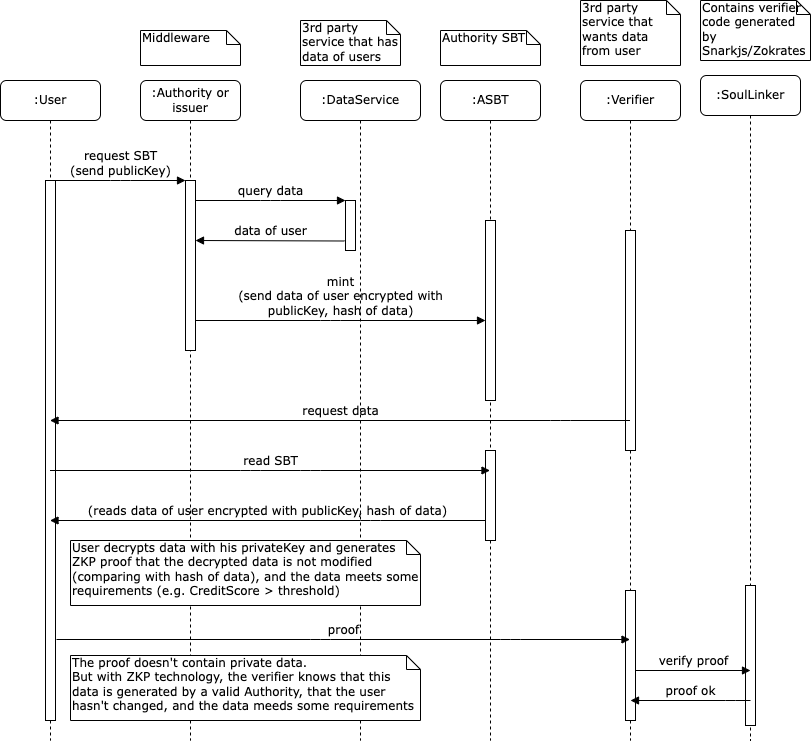
\includegraphics[width=0.5\textwidth]{sequence-digram.png}
    \caption{Masa zkpSBT sequence diagram}
  \end{figure}
\subsubsection{Key components}
\begin{enumerate}
    \item Structures:
    \begin{enumerate}[label*=\arabic*.]
      \item \texttt{EncryptedData}: A structure that contains the encryption-related data such as initialization vector (IV), ephemeral public key, ciphertext, and message authentication code (MAC).
      \item \texttt{SBTData}: A structure that stores the hash data and the encrypted data (EncryptedData) associated with a specific token ID.
    \end{enumerate}
    \item Mappings:
    \begin{enumerate}[label*=\arabic*.]
      \item \texttt{sbtData}: A mapping that associates a token ID with its corresponding SBTData.
    \end{enumerate}
    \item Constructor:
    \begin{enumerate}[label*=\arabic*.]
      \item Initializes the \texttt{zkSBT} contract by inheriting from the \texttt{MasaSBTSelfSovereign} or \texttt{MasaSBTAuthority} contracts, and sets the necessary parameters such as \texttt{admin}, \texttt{name}, \texttt{symbol}, \texttt{baseTokenURI}, \texttt{SoulboundIdentity} contract \texttt{address}, and payment parameters.
    \end{enumerate}
    \item Functions:
    \begin{enumerate}[label*=\arabic*.]
      \item \texttt{getHashData(uint256 tokenId)}: A function to retrieve the hash data associated with a specific token ID.
      \item \texttt{getEncryptedData(uint256 tokenId)}: A function to retrieve the encrypted data associated with a specific token ID, encrypted with the public key of the owner of that token.
      \item \texttt{mint(address to, address authorityAddress, uint256 signatureDate, bytes calldata hashData, EncryptedData calldata encryptedData, bytes calldata signature)}: A function that mints a new SBT, verifies the caller's authorization and stores the provided SBTData. This function emits a MintedToAddress event.
    \end{enumerate}
    \item Events:
    \begin{enumerate}[label*=\arabic*.]
      \item \texttt{MintedToAddress}: An event emitted when a new SBT is minted, containing tokenId, recipient address, authority address, signature date, payment method, and mint price.
    \end{enumerate}
  \end{enumerate}

  \subsubsection{zkpSBT}

  \begin{verbatim}
    // SPDX-License-Identifier: MIT
    pragma solidity ^0.8.7;
    /// @title ZKP SBT
    /// @author Masa Finance
    /// @notice Soulbound token implementing ZKP
    abstract contract ZKPSBT {
        struct EncryptedData {
            bytes iv; // IV
            bytes ephemPublicKey; // ephemPublicKey
            bytes cipherText; // ciphertext
            bytes mac; // mac
        }
        // Struct to store the encrypted data with the public key of the owner of the SBT
        struct SBTData {
            bytes hashData; // hash of ownerAddress+creditScore without encryption, used to verify the data
            EncryptedData encryptedData; // encrypted data with the public key of the owner of the SBT
        }
        // tokenId => SBTData
        mapping(uint256 => SBTData) public sbtData;
        function getHashData(uint256 tokenId) external view returns (bytes memory) {
            return sbtData[tokenId].hashData;
        }
        function getEncryptedData(
            uint256 tokenId
        ) external view returns (EncryptedData memory) {
            return sbtData[tokenId].encryptedData;
        }
    }
    \end{verbatim}
\subsubsection{Example use cases for the zkSBT (Zero-Knowledge Soulbound Token)}
\begin{enumerate}
\item Secure Identity Verification: A user can store their encrypted personal identification information (e.g., passport number, social security number) within a zkSBT. When interacting with a third-party service that requires identity verification, the user can share their zkSBT without revealing their actual personal information, while the third party can verify the authenticity of the data using zero-knowledge proofs.
\item Privacy-Preserving Credit Scoring: A credit scoring service can store users' encrypted credit score data within zkSBTs. When a user applies for a loan, they can share their zkSBT with the lending institution. The institution can verify the user's creditworthiness without accessing the actual credit score data, thereby preserving the user's privacy.
\item Decentralized Reputation Systems: In a web3 ecosystem, users can store their encrypted reputation data, such as reviews or ratings from decentralized applications (dApps), within zkSBTs. When interacting with dApps or services that require reputation-based access or decision-making, users can share their zkSBT without revealing specific details about their interactions. The dApp or service can verify the authenticity and overall reputation score using zero-knowledge proofs, ensuring user privacy.
\item Secure Voting: In a decentralized voting system, voters can store their encrypted votes within zkSBTs. Election authorities can use zero-knowledge proofs to verify the validity of votes without revealing the actual vote content, thereby ensuring voter privacy and the integrity of the voting process.
\item Private Asset Ownership: Users can store encrypted records of their asset ownership (e.g., real estate, vehicles) within zkSBTs. When required to prove ownership, users can share their zkSBT with relevant authorities, allowing them to verify ownership without revealing the specific details of the assets.
\end{enumerate}
These use cases demonstrate the versatility and potential of the zkSBT contract in enabling privacy-preserving and secure storage of private data on the EVM blockchain in the web3 ecosystem.


\section{Masa Protocol}
Developers using the Masa Protocol, and its infrastructure which includes SDKs and developers tools such as the Masa CLI\cite{cli}, pay a fee that goes directly to the protocol treasury for distribution back to node operators and for maintaining the protocol. Fees are collected on-chain in MASA tokens and native blockchain tokens for the following actions:
\begin{enumerate}
    \item Deploying a Soulname, ASBT, SSSBT, or zkSBT contract using Masa infrastructure
    \item Minting a Soulname, ASBT, SSBT, or zkSBT
    \item Requesting permission to read private data
    \item Querying and relaying private data 
    \item Crosschain oracle services
    \item EIP-4337 services, including SDK interactions
  \end{enumerate}
An example Masa Green 2FA mint transaction with a \$1.00 fee can be seen here\cite{polygon} - \$1.00 in MATIC is transferred to the Masa Protocol multi-sig wallet\cite{polygon-multisig}.
\subsection{Oracle Network for Identity Data}
The Masa Protocol employs a set of oracle nodes to govern decentralized identity data, drawing inspiration from Chainlink's\cite{chainlink} decentralized oracle network. These oracle nodes are responsible for the following tasks:
\begin{itemize}
\item Retrieving encrypted identity data from off-chain data providers, such as government databases, credit bureaus, or private identity verification services.
\item Validating data to ensure its accuracy, reliability, and timeliness as a decentralized authority.
\item Relaying and maintaining the state of identity data in smart contracts deployed on the blockchain, enabling the execution of various identity-related tasks, such as updating an off-chain credit score associated with an on-chain smart contract or zkSBT.
\item Relaying on-chain identity-permissions passports to the SoulLinker contract to enable encrypted off-chain private data to be updated in smart contracts ensuring decentralized governance of private off-chain data. 
\end{itemize}
Additionally, the oracle nodes integrate key components from EIP-4337, such as account abstraction, bundlers, and paymasters, to provide a superior way to manage identity through a more efficient and user-friendly web3 experience.
\begin{enumerate}
\item Account abstraction: Masa's Oracle network enables users to use smart contracts as their accounts, simplifying the user experience and offering additional functionality such as multi-sig verification, sponsored transactions, and enhanced security features and account recovery for SBT holders.
\item Bundler: The Masa Protocol incorporates a bundler that is compatible with the ERC-4337 standard. The Masa bundler helps to manage gasless transactions for SSSBTs, ASBTs, and on-chain permissions of data through batched transactions, and other advanced features, making the Masa Protocol more accessible and versatile for its users.
\item Paymaster: Masa's Oracle network has paymasters to facilitate transaction sponsorship, allowing users to execute gasless transactions and enabling third-party mechanisms to pay for transaction fees. This offers users the flexibility to pay transaction fees using ERC-20 tokens or to have fees sponsored by the Masa protocol, enhancing the overall user experience.
\end{enumerate}
With the Masa Protocol's decentralized oracle network, the protocol can effectively govern identity data while providing a more efficient and user-friendly experience through fully decentralized infrastructure.

\subsection{Account abstraction}
Account abstraction has been pioneered by the Ethereum Foundation and EIP-4337\cite{eip4337}. EIP-4337 decouples the traditional relationship between a user's externally owned account (EOA) and the associated private key. In conventional blockchain systems, users interact with the network using EOAs, which are controlled by an external private key. While this model has been widely adopted, it can present a barrier to entry for some users due to its reliance on a deep understanding of blockchain mechanics and public key, and private key cryptography.
\\
\newline
In contrast, account abstraction allows users to interact with the network through smart contract accounts (smart accounts), which offer more flexibility and programmability compared to EOAs. By leveraging the expressive power of smart contracts, account abstraction enables the implementation of custom transaction verification logic, such as multi-signature schemes, while simultaneously offering additional features, such as sponsored transactions, enhanced security measures, and atomic multi-operations.
\\
\newline
Sponsored transactions, for instance, provide users with the option to pay for transaction fees in tokens other than the blockchain's native currency or have the fees subsidized by a third party – a Paymaster. This feature can help lower barriers to entry and enhance the overall user experience by abstracting gas fees from the user experience. Additionally, account abstraction allows for the integration of advanced security features, such as social recovery mechanisms, time-locks, and biometrics which can further protect users from malicious actors or loss of private keys.
\\
\newline
Furthermore, atomic multi-operations enable users to conduct multiple, interrelated transactions in a single step, resulting in reduced complexity and lower transaction costs. This capability allows for more intuitive and streamlined interactions with decentralized applications and smart contracts.

\subsection{Oracle Network and Account Abstraction Incentive Mechanisms}
The Masa Protocol utilizes its decentralized oracle network to establish incentive mechanisms that encourage participation from node operators, bundlers, and paymasters. 

\subsubsection{Incentive Mechanisms}
Node Operator Incentives
\begin{enumerate}
\item Payment for Oracle services: Node operators are compensated with Masa Protocol's native tokens as well as other payments received in stablecoins, native blockchain assets – such as ETH, MATIC, or BNB – for providing Oracle services, including retrieving, validating, and maintaining the state of identity data in smart contracts.
\item Reputation and performance-based incentives: Node operators with a history of accurate and reliable performance are rewarded with additional incentives, encouraging them to maintain high-quality services.
\end{enumerate}
Bundler Incentives

\begin{enumerate}
\item Fee distribution: Bundlers receive a portion of the transaction fees for processing gasless transactions, batched transactions, and other advanced features within the Masa Protocol.
\item Performance-based incentives: Bundlers that demonstrate efficient and reliable transaction processing may receive additional rewards to promote continued high-quality performance.
\end{enumerate}
Paymaster Incentives

\begin{enumerate}
\item Compensation for transaction sponsorship: Paymasters are rewarded with Masa Protocol's native tokens for facilitating transaction sponsorship and enabling gasless transactions for users.
\item Reputation-based incentives: Paymasters with a proven track record of reliable and efficient transaction sponsorship are granted additional incentives to encourage the provision of high-quality services.
\end{enumerate}
By implementing these incentive mechanisms, the Masa Protocol aims to create a sustainable and reliable decentralized oracle network that can effectively govern identity data while providing an efficient and user-friendly experience through a fully decentralized infrastructure.

\section{Masa Protocol Governance}
\subsection{Token-based Voting Rights}
\begin{enumerate}
\item Masa token holders have the ability to participate in protocol governance decisions by proposing and voting on various protocol upgrades, changes, and improvements. 
\item At launch, the weight of a token holder's vote is proportional to the amount of Masa tokens they hold, which ensures that those with a larger stake in the protocol have a greater influence on its governance. 
\end{enumerate}
\subsection{Staking and Delegation}
\begin{enumerate}
\item Masa token holders can choose to stake their tokens to secure the network and earn staking rewards. Stakers play a vital role in maintaining the network's security and stability.
\item Token holders who do not wish to actively participate in staking can delegate their tokens to professional node operators, sharing the staking rewards while still contributing to the network's security.
\item Oracle node operators who wish to function as bundlers and paymasters must stake tokens in the Masa Prototocol bundler and paymaster smart contracts.
\end{enumerate}
\subsection{Incentivizing Network Participants}
\begin{enumerate}
\item The Masa token serves as the primary means of incentivizing various network participants, such as node operators, bundlers, and paymasters, to provide high-quality services within the Masa Protocol.
\item By distributing Masa tokens as rewards for Oracle network node operators, the protocol ensures that these participants remain invested in the overall success and growth of the ecosystem.
\end{enumerate}
\subsection{Protocol Treasury}
\begin{enumerate}
\item A portion of the Masa tokens is allocated to a protocol treasury, which is governed by the token holders. The treasury funds can be utilized for various purposes, such as network upgrades, development grants, and ecosystem growth initiatives.
\item Token holders can vote on proposals for using treasury funds, ensuring that the allocation of resources is aligned with the best interests of the Masa Protocol community.
\end{enumerate}

By incorporating the Masa token as the backbone of the protocol's governance structure, the Masa Protocol ensures that all stakeholders have a vested interest in the network's success and can actively participate in shaping its future. This decentralized approach to governance fosters a strong, inclusive, and sustainable ecosystem.
\section{Conclusion}
In this paper, we have presented the first version of the Masa Protocol; a groundbreaking solution for decentralized identity infrastructure tailored to the needs of web3 communities. Central to our vision to bring humanity on-chain are Soulbound Tokens (SBTs), and Zero-Knowledge Soulbound Tokens (zkSBTs).
\\
\newline
SBTs are highly composable on-chain identifiers that can be applied to functional use cases in building web3 communities, such as user acquisition, gamified community engagement, and user verification. zkSBTs serve as the foundation for secure and privacy-preserving digital identities, employing zero-knowledge proofs to maintain the confidentiality of off-chain data while still facilitating verifiable on-chain interactions. This is made possible through the Masa Protocol's decentralized oracle network, which retrieves, validates, and maintains identity data, ensuring the accuracy and reliability of information while enabling a plurality of identity-related use cases.
\\
\newline
Moreover, the Masa Protocol incorporates key components of EIP-4337, such as account abstraction, bundlers, and paymasters. This allows for a superior and user-friendly web3 identity experience, with features like social key recovery, private key rotation, sponsored transactions, and enhanced security for SBT holders. The bundler and paymaster systems also contribute to making the Masa Protocol accessible to the next billion users through smart accounts and third-party transaction fee sponsorship.
\\
\newline
As web3 communities continue to evolve, the Masa Protocol is set to revolutionize identity infrastructure in web3. By delivering a robust, user-friendly, and privacy-centric infrastructure, the Masa Protocol cements its role as the leader in the identity infrastructure for user-oriented blockchains, web3 applications, and their communities.
\appendix
\section{Appendix A: EIP-SBT}
\label{app.eipsbt}
\begin{verbatim}
  // SPDX-License-Identifier: Apache-2.0
pragma solidity ^0.8.7;

import "@openzeppelin/contracts/utils/introspection/ERC165.sol";
import "@openzeppelin/contracts/utils/Context.sol";
import "@openzeppelin/contracts/utils/Strings.sol";

import "./ISBT.sol";
import "./extensions/ISBTMetadata.sol";

/// @title SBT
/// @author Masa Finance
/// @notice Soulbound token is an NFT token that is not transferable.
contract SBT is Context, ERC165, ISBT, ISBTMetadata {
    using Strings for uint256;

    // Token name
    string private _name;

    // Token symbol
    string private _symbol;

    // Mapping from token ID to owner address
    mapping(uint256 => address) private _owners;

    // Mapping owner address to token count
    mapping(address => uint256) private _balances;

    /**
     * @dev Initializes the contract by setting a `name` and a `symbol` to the token collection.
     */
    constructor(string memory name_, string memory symbol_) {
        _name = name_;
        _symbol = symbol_;
    }

    /**
     * @dev See {IERC165-supportsInterface}.
     */
    function supportsInterface(bytes4 interfaceId)
        public
        view
        virtual
        override(ERC165, IERC165)
        returns (bool)
    {
        return
            interfaceId == type(ISBT).interfaceId ||
            interfaceId == type(ISBTMetadata).interfaceId ||
            super.supportsInterface(interfaceId);
    }

    /**
     * @dev See {ISBT-balanceOf}.
     */
    function balanceOf(address owner)
        public
        view
        virtual
        override
        returns (uint256)
    {
        require(owner != address(0), "SBT: address zero is not a valid owner");
        return _balances[owner];
    }

    /**
     * @dev See {ISBT-ownerOf}.
     */
    function ownerOf(uint256 tokenId)
        public
        view
        virtual
        override
        returns (address)
    {
        address owner = _owners[tokenId];
        require(owner != address(0), "SBT: invalid token ID");
        return owner;
    }

    /**
     * @dev See {ISBTMetadata-name}.
     */
    function name() public view virtual override returns (string memory) {
        return _name;
    }

    /**
     * @dev See {ISBTMetadata-symbol}.
     */
    function symbol() public view virtual override returns (string memory) {
        return _symbol;
    }

    /**
     * @dev See {ISBTMetadata-tokenURI}.
     */
    function tokenURI(uint256 tokenId)
        public
        view
        virtual
        override
        returns (string memory)
    {
        _requireMinted(tokenId);

        string memory baseURI = _baseURI();
        return
            bytes(baseURI).length > 0
                ? string(abi.encodePacked(baseURI, tokenId.toString()))
                : "";
    }

    /**
     * @dev Base URI for computing {tokenURI}. If set, the resulting URI for each
     * token will be the concatenation of the `baseURI` and the `tokenId`. Empty
     * by default, can be overridden in child contracts.
     */
    function _baseURI() internal view virtual returns (string memory) {
        return "";
    }

    /**
     * @dev Returns whether `spender` is allowed to manage `tokenId`.
     *
     * Requirements:
     *
     * - `tokenId` must exist.
     */
    function _isOwner(address spender, uint256 tokenId)
        internal
        view
        virtual
        returns (bool)
    {
        address owner = SBT.ownerOf(tokenId);
        return (spender == owner);
    }

    /**
     * @dev Returns whether `tokenId` exists.
     *
     * Tokens can be managed by their owner.
     *
     * Tokens start existing when they are minted (`_mint`),
     * and stop existing when they are burned (`_burn`).
     */
    function _exists(uint256 tokenId) internal view virtual returns (bool) {
        return _owners[tokenId] != address(0);
    }

    /**
     * @dev Mints `tokenId` and transfers it to `to`.
     *
     * WARNING: Usage of this method is discouraged, use {_safeMint} whenever possible
     *
     * Requirements:
     *
     * - `tokenId` must not exist.
     * - `to` cannot be the zero address.
     *
     * Emits a {Mint} event.
     */
    function _mint(address to, uint256 tokenId) internal virtual {
        require(to != address(0), "SBT: mint to the zero address");
        require(!_exists(tokenId), "SBT: token already minted");

        _beforeTokenTransfer(address(0), to, tokenId);

        _balances[to] += 1;
        _owners[tokenId] = to;

        emit Mint(to, tokenId);

        _afterTokenTransfer(address(0), to, tokenId);
    }

    /**
     * @dev Destroys `tokenId`.
     *
     * Requirements:
     * - `tokenId` must exist.
     *
     * Emits a {Burn} event.
     */
    function _burn(uint256 tokenId) internal virtual {
        address owner = SBT.ownerOf(tokenId);

        _beforeTokenTransfer(owner, address(0), tokenId);

        _balances[owner] -= 1;
        delete _owners[tokenId];

        emit Burn(owner, tokenId);

        _afterTokenTransfer(owner, address(0), tokenId);
    }

    /**
     * @dev Reverts if the `tokenId` has not been minted yet.
     */
    function _requireMinted(uint256 tokenId) internal view virtual {
        require(_exists(tokenId), "SBT: invalid token ID");
    }

    /**
     * @dev Hook that is called before any token minting/burning
     *
     * Calling conditions:
     *
     * - When `from` and `to` are both non-zero, ``from``'s `tokenId` will be
     * transferred to `to`.
     * - When `from` is zero, `tokenId` will be minted for `to`.
     * - When `to` is zero, ``from``'s `tokenId` will be burned.
     * - `from` and `to` are never both zero.
     *
     * To learn more about hooks, head to xref:ROOT:extending-contracts.adoc#using-hooks[Using Hooks].
     */
    function _beforeTokenTransfer(
        address,
        address,
        uint256
    ) internal virtual {}

    /**
     * @dev Hook that is called after any minting/burning of tokens
     *
     * Calling conditions:
     * - when `from` and `to` are both non-zero.
     * - `from` and `to` are never both zero.
     *
     * To learn more about hooks, head to xref:ROOT:extending-contracts.adoc#using-hooks[Using Hooks].
     */
    function _afterTokenTransfer(
        address,
        address,
        uint256
    ) internal virtual {}
}
\end{verbatim}

\bibliographystyle{unsrtnat}
\bibliography{sample}

\end{document}